
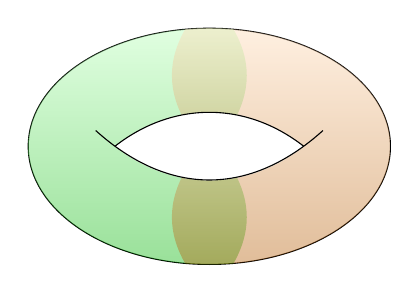
\begin{tikzpicture}
\path[draw, clip] (0,0) ellipse (2.3cm and 1.5cm);

\begin{scope}
\clip(0.3, 1.5) to [bend left] (0.3, 0.3) -- (0.3, -0.3) to [bend left] (0.3, -1.5) -- (-2.3, -1.5) -- (-2.3, 1.5) -- cycle;

\shade[top color = green!30!white, bottom color = green!70!black, opacity = 0.4] (-2.3, -1.5) rectangle (0.5, 1.5);
\end{scope}

\begin{scope}
\clip(-0.3, 1.5) to [bend right] (-0.3, 0.3) -- (-0.3, -0.3) to [bend right] (-0.3, -1.5) -- (2.3, -1.5) -- (2.3, 1.5) -- cycle;

\shade[top color = orange!30!white, bottom color = orange!70!black, opacity = 0.4] (2.3, -1.5) rectangle (-0.5, 1.5);
\end{scope}


\fill[white] (1.2, 0) to[bend right = 38] (-1.2, 0) to[bend right = 38] (1.2, 0);
\draw (1.2, 0) to[bend right = 38] (-1.2, 0);
\draw[shorten >= -0.3cm, shorten <= -0.3cm] (1.22, 0) to[bend left = 42] (-1.22, 0);

\end{tikzpicture}
